\chapter{Méthodes itératives pour les systèmes linéaires}

On sait aujourd'hui résoudre numériquement des systèmes linéaires de l'ordre du million d'inconnues (et d'équations). Pour des \textbf{systèmes creux}, c'est-à-dire lorsque la matrice du système possède beaucoup de coefficients nuls, on arrive à une centaine de millions d'inconnues.
Les \textbf{systèmes pleins} font appel à des \textbf{méthodes directes}, qui donnent la solution exacte (aux erreurs d'arrondi près) en un nombre fini d'itérations, et seront décrites dans un chapitre ultérieur.

Pour les \textbf{très grands systèmes creux\footnote{Exemple : discrétisation par différences finies de problèmes aux limites pour des équations aux dérivées partielles ...}}
on utilise des \textbf{méthodes itératives}, où on construit une suite de vecteurs qui convergent vers la solution.

L'intérêt est que \textbf{ces méthodes ne manipulent pas la matrice}, mais seulement une fonction qui définit une suite par récurrence.

\begin{fdef}
    Soit $A \in M_n(\R)$ inversible et $b \in \R^n$. On appelle méthode itérative de résolution du système linéaire $Ax=b$, ($x \in \R^n$) 
    une méthode qui construit une suite récurrente $(x_k)_{k\geq0}$
    telle que $$(x_k \underset{k\to +\infty}{\longrightarrow} x) \Rightarrow Ax=b$$
    Une méthode itérative est convergente si $x_k \underset{k\to +\infty}{\longrightarrow}x$ pour toute condition initiale $x_0 \in \R^n$
\end{fdef}

\underline{Tests d'arrêt typiques :}

% Pour les listes à puces, met un point noir en Énum
\renewcommand{\labelitemi}{\textbullet}
\begin{itemize}
    \item $\frac{\|Ax_k - b \|}{\|b\|} < \varepsilon$ (norme du ``résidu'' / norme de b).

        Noter que : 
        \begin{align*} \frac{\|x_k-x\|}{\|x\|} 
            = \frac{\|A^{-1}(Ax_k-b)\|}{\|x\|} 
            & \leq \|A^{-1}\| \frac{\|b\|}{\|x\|}\varepsilon 
            \\ & \leq \|A^{-1}\| \|A\| \varepsilon, 
            \; \mbox{peut-être grand !}\end{align*}

\end{itemize}


Nous allons décrire ici des méthodes itératives avec ``splitting'' de A.


\section{Description générale :}

On considère ici le système
\begin{equation}
    \label{eq:eqdiff}
    Ax = b
\end{equation} 
où $A \in M_n(\R)$, $x \in \R^n$ et $b \in \R^n$. On suppose que la matrice $A$ est inversible.


On considère une décomposition de A (``splitting'') $A=M-N$ avec $M$ inversible et on considère l'itération :

\begin{equation}
\left\lbrace
\begin{array}{ccc}
    Mx_{k+1} & = & Nx_k + b\\
    \\
    x_0 \in \R^n
    \label{eq:2}
\end{array}\right.
\end{equation}

Si $x_k \to x$ quand $k \to +\infty$ alors $Mx = Nx + b$, càd $x$ est solution de \reff{eq:eqdiff}.

Le choix du splitting est très important pour la performance de la méthode :
\begin{itemize}
    \item Bien sûr la méthode doit être convergente (voir plus loin)
    \item On doit choisir $M$ de telle sorte que le système \reff{eq:2} soit beaucoup plus facile à résoudre que \reff{eq:eqdiff} (il faut résoudre \reff{eq:2} à chaque étape de l'itération).

        \underline{Exemples :} $M$ diagonale ou triangulaire, diagonale ou triangulaire par blocs.
\end{itemize}

Étudions les conditions de convergence de \reff{eq:2}.

\begin{fdef}
    Étant donné $A \in M_n(\C)$, on note $S_p(A)$ l'ensemble des valeurs propres de $A$ (ou ``spectre de A''). On appelle rayon spectral de $A$ et on note $\rho(A)$ :
\[
    \rho (A) = \underset{\lambda \in S_p(A)}{\Max|\lambda|}
\]
\end{fdef}

\begin{ftheo}
    La méthode \reff{eq:2} converge si et seulement si $$\rho(M^{-1}N) < 1$$
\end{ftheo}

La preuve complète de ce résultat sera étudiée en TD. Ici nous allons simplement montrer que $\rho(M^{-1}N)<1 \Rightarrow $ convergence de \reff{eq:2}, en admettant pour cela deux résultats.

\vspace{1cm}

\begin{ftheo}[de l'application contractante (dans $\R^n$) ]
    Soit $E$ un sous-ensemble de $\R^n$ fermé (et non vide). On considère une norme $\| \, \|$ sur $\R^n$.

    Soit $F : E \rightarrow E$ une application contractante, càd pour laquelle il existe $\alpha \in [0,1[$ tel que :
\[
    \| F(x) - F(y) \| \leq \alpha \| x-y \| \mbox{,} \: \: \forall x,y \in E
\]

    Alors il existe un unique $x^* \in E$ tel que $F(x^*)=x^*$ (càd $F$ admet un unique point fixe dans E). De plus, pour tout $x_0 \in E$, la suite définie par :
\[
    x_{k+1} = F(x_k)
\]
converge vers $x^*$, avec
\begin{equation}
    \| x^* - x_k \| \leq \frac{\alpha^k}{1 - \alpha} \| x_1 - x_0 \|
    \label{eq:3}
\end{equation}

Le système \reff{eq:2} s'écrit :

\begin{equation}
\left\lbrace
\begin{array}{c}
    \boxed{x_{k+1} = M^{-1}N x_k + M^{-1} b}\\
    \\
    x_0 \in \R^n
    \label{eq:5}
\end{array}\right.
\end{equation}

\end{ftheo}

\begin{remark}
   Théorème encore appelé ``Théorème du point fixe de Banach''. Le théorème reste vrai lorsque $E$ est un espace métrique complet.
\end{remark}

\begin{ftheo}[cf TD pour la démonstration]
    Soit $A \in M_n(\C)$ et $\varepsilon > 0$. Il existe une norme $\| \, \|$ sur $\C^n$ telle que :
\[
    \underbrace{\|A\|}_
    \text{\parbox[]{2cm}{norme sur $M_n(\C)$ induite par la norme $\| \, \|$ de $C^n$}}
        :=  \underset{\|x\|=1}{\Sup} \|Ax\| \leq \rho(A) + \varepsilon
\]
  
\end{ftheo}

Si $\rho (M^{-1}N) < 1$, il existe donc une norme matricielle induite telle que $\| M ^{-1} N \| \leq \rho (M^{-1} N) + \varepsilon < 1$. Alors :
\[
    \| F(x) - F(y) \| = \| M^{-1} N (x-y) \| \leq \underbrace{\| M^{^-1}N \|}_{< 1} \| x-y \|
\]

Donc $F : \R^n \rightarrow \R^n$ est une contraction.

Donc $\forall x_0 \in R^n$, la suite définie par \reff{eq:5} converge vers une limite $x \in \R^n$ unique, solution de $x = M^{-1}Nx+M^{-1}b$, c'est-à-dire $Ax=b$.

% Je ne sais pas comment présenter ces points
\vspace{1cm}
\underline{Vitesse de convergence :} Plus $\rho(M^{-1}N)$ est petit, plus $\|M^{-1}N\|$ peut être choisie petite et plus la convergence est rapide.
En effet, d'après \reff{eq:3} :
\[
    \|x-x_k\| \leq \frac{\|M^{-1}N\|^k}{1-\|M^{-1}N\|}\|x_1-x_0\|
\]

\vspace{1cm}
\underline{Exemple de splitting : } (peu utilisé)
\[
    M = \frac{1}{\alpha}I, \qquad N = \frac{1}{\alpha}I - A \qquad \Longrightarrow \qquad x_{k+1} = (I - \alpha A)x_k + \alpha b
\]
(méthode de Richardson stationnaire, ou du gradient à pas fixe)

Elle converge si et seulement si $\forall \lambda \in Sp(A), |1-\alpha \lambda | < 1$, c'est-à-dire toutes les valeurs propres de A se trouvent dans le disque (ouvert) de centre $(\frac{1}{\alpha}, 0)$ et de rayon $\left| \frac{1}{\alpha} \right|$.

\section{Méthode de Jacobi}
On pose dans le schéma \reff{eq:2} :
\[
    M = D \mbox{ avec $D$ diagonale et } d_{ii}=a_{ii}, \qquad N=D-A
\]

On a donc :
\begin{equation}
D \cdot x_{k+1} = (D-A) \cdot x_k + b
\end{equation}
\begin{equation}
x_{k+1} = (I - D^{-1}A) \cdot x_k + D^{-1} b
\end{equation}

\begin{remark}
    Cela suppose $a_{ii} \ne 0 \; \forall i$ (si cette condition n'est pas vérifiée on peut permuter des lignes de $A$).
\end{remark}

En notant $x_k = (x^{(k)}_1,\dots,x^{(k)}_n)$ on obtient pour $i=1 \cdots n$ :
\begin{equation}
x^{(k+1)}_i = - \sum_{j \ne i}\frac{a_{ij}}{a_{ii}} \cdot x_j^{(k)} + \frac{b_i}{a_{ii}}
\end{equation}

\begin{ftheo}
    Si $A$ est à diagonale strictement dominante ($\rightarrow a_{ii}>0$ et $D$ inversible) alors la méthode de Jacobi converge.
\end{ftheo}

La démonstration sera vue en TD. On montre que le rayon spectral $\rho(J)$ de la matrice de Jacobi $J = D^{-1}N = D^{-1}(D-A) = I - D^{-1}A$ est $< 1$.

Nous avons rencontré ce type de matrices pour la discrétisation de problèmes aux limites dans le $1^{er}$ chapitre du cours.

\section{Méthode de Gauss-Seidel}

On suppose $a_{ii} \ne 0$, $\forall i = 1 \cdots n$.
\begin{itemize}
\item Méthode souvent plus rapidement convergente que celle de Jacobi
\item + économique en terme de stockage : un seul vecteur à stocker pour le calcul de l'itéré suivant
\item Converge pour les matrices symétriques définies positives (pas le cas pour Jacobi)
\end{itemize}

On pose $A = L + D + U$ avec :

\[
   L =
   \begin{pmatrix}
        0        & \cdots & 0      \\
        \vdots   & \ddots & \vdots \\
        a_{ij}(i>j)      & \cdots & 0
   \end{pmatrix}
   , D =
   \begin{pmatrix}
       a_{11} & \cdots                      & 0      \\ 
       \vdots & a_{ii}\hspace{-0.5cm}\ddots & \vdots \\ 
       0      & \cdots                      & a_{nn}
   \end{pmatrix}
   , U =
   \begin{pmatrix}
        0        & \cdots & a_{ij}(j>i)     \\
        \vdots   & \ddots & \vdots \\
        0        & \cdots & 0
   \end{pmatrix}
\]

Dans la méthode de Gauss-Seidel, on fixe :
\[
    M = L + D, \; N = -U
\]
\[
    \Rightarrow A = M - N
\]

La méthode s'écrit donc :
\[
    Dx_{k+1} = -Lx_{k+1}-Ux_k + b
\]
En notant $x_k = (x^{(k)}_1,\dots,x^{(k)}_n)$ on obtient pour $i = 1 \cdots n$ :
\[
    a_{ii}x^{(k+1)}_i = - \sum_{j<i}a_{ij}x_j^{(k+1)} - \sum_{(j>i)}a_{ij}x_j^{(k)} + b_i
\]

\begin{ftheo}
    Si $A$ est à diagonale strictement dominante alors la méthode de Gauss-Seidel converge.
\end{ftheo}

\begin{ftheo}
    Si $A$ est symétrique définie positive (SDP) alors la méthode de Gauss-Seidel converge.
\end{ftheo}

A est SDP $\Leftrightarrow$ $^txAx > 0, \forall x \ne 0$


\newpage

\section{Méthode de relaxation}

Les méthodes de Jacobi et Gauss-Seidel ne sont guère utilisées. On leur préfère la méthode de relaxation.

La méthode SOR (``successive over-relaxation'', ou ``méthode de relaxation'', environ 1950) généralise Gauss-Seidel en introduisant un \textbf{paramètre de relaxation $\omega$} $\ne 0$,
que l'on ajuste afin d'accélérer la convergence de la méthode (avec un gain généralement très important si $\omega$ est bien choisi).

\begin{center}
$\forall i = 1 \cdots n$ :
\end{center}
\begin{equation}
\left\lbrace
\begin{array}{ccc}
    a_{ii} \cdot \tilde{x}_i^{(k+1)} & = & -\sum_{j<i} a_{ij} \cdot x_j^{(k+1)} - \sum_{j>i}a_{ij} \cdot x_j^{(k)} + b_i\\
    x_i^{(k+1)} & = & \omega \cdot \tilde{x_i}^{(k+1)} + (1-\omega) \cdot x_i^{(k)}
    \label{eq:4}
\end{array}\right.
\end{equation}

\begin{center}
\underline {$\omega = 1$} $\Rightarrow$ Gauss-Seidel
\end{center}
% (Gauss-Seidel correspond à $\omega = 1$)


\subsection {Reformulation matricielle}
\begin{equation*}
A = L + D + U
\end{equation*}

On multiplie la seconde ligne par $a_{ii}$ et on écrit matriciellement le système pour $i = 1 \cdots n$ :

\[
    D \cdot x^{(k+1)}= - \omega L x^{(k+1)} - \omega U x^{(k)} + \omega b + (1-\omega) D x^{(k)}
\]

soit

\[
    (\frac{1}{\omega}D + L) \cdot x^{(k+1)} = \left [\frac{1-\omega}{\omega} D - U \right] x^{(k)} + b
\]

Le schéma s'écrit :
\[
    M \cdot x^{(k+1)} = N \cdot x^{(k)} + b
\]
\[
    M = \frac{1}{\omega}D + L, N = \frac{1-\omega}{\omega} D - U
\]
\[
    \Rightarrow M - N = L + D + U = A
\]

Soit :
\[
    \mathcal{L}_{\omega} = (\frac{1}{\omega}D + L)^{-1}(\frac{1-\omega}{\omega}D - U) = M^{-1} \cdot N
\]
La méthode de relaxation converge si $\rho(\mathcal{L}_{\omega}) < 1$ et plus $\rho$ est petit, plus la convergence est rapide.

$\newline$
On suppose $a_{ii} \ne 0$, $\forall i = 1 \cdots n$ (comme précédemment).
\begin{ftheo}
~
    \begin{enumerate}
        \item
            Une condition nécessaire pour que la méthode de relaxation converge est $\omega \in ]0,2[$

        \item
            Si A est symétrique définie positive, alors $\forall \omega \in ]0,2[$ la méthode de relaxation converge.
    \end{enumerate}
\end{ftheo}

% 1) [demo en TD]

\begin{ftheo}
    Si A est à diagonale strictement dominante et $\omega \in ]0,1]$ alors la méthode de relaxation converge.
\end{ftheo}

\begin{rappel}
    $A$ est symétrique définie positive si $A$ est symétrique, $^txAx = 0 \Rightarrow x = 0$, et $\forall x \in \R^n, {}^t\!xAx \geq 0$
\end{rappel}

\begin{coroll}
    Si $A$ est symétrique définie positive, alors la méthode de Gauss-Seidel converge.
    Nous avons rencontré ce type de matrices pour la discrétisation des problèmes aux limites dns le $1^{er}$ chapitre du cours (paragraphe 2), cas où la fonction $p$ est identiquement nulle.
\end{coroll}

\begin{remark}
    \begin{enumerate}
        \item Il y a des exemples où $A$ est symétrique définie positive et où la méthode de Jacobi n'est pas convergente.
        \item Si A est tridiagonale ($a_{ij}=0$ si $\abs{i-j}>1$) et $D$ inversible, on peut montrer que $\rho(\mathcal{L}_1)=\rho(J)^2$, avec $J = I - D^{-1} A$. Donc la méthode de Gauss-Seidel converge si et seulement si celle de Jacobi converge (et Gauss-Seidel converge plus vite).
        \item  Pour quelques types de matrices, on connaît la valeur de $\omega$ qui minimise $\rho (\mathcal{L}_{\omega})$.
            Pour $A$ tridiagonale (avec $D$ inversible), et si les valeurs propres de $J$ sont réelles, alors le paramètre de relaxation optimal dans SOR (c'est-à-dire la valeur de $\omega$ qui minimise $\rho (\mathcal{L}_{\omega})$) est > 1 (donc Gauss-Seidel ne donne pas la vitesse optimale de convergence).
        \item Pour optimiser empiriquement le choix de $\omega$ dans SOR, on peut évaluer le facteur de contractivité $\frac{\| x_{k+1} - x_k\|}{\| x_k - x_{k-1}\|}$ à partir du moment où $\|x_{k+1}-x_{k}\|$ décroît vers 0.
    \end{enumerate}
\end{remark}

\begin{figure}[h]
    \centering
    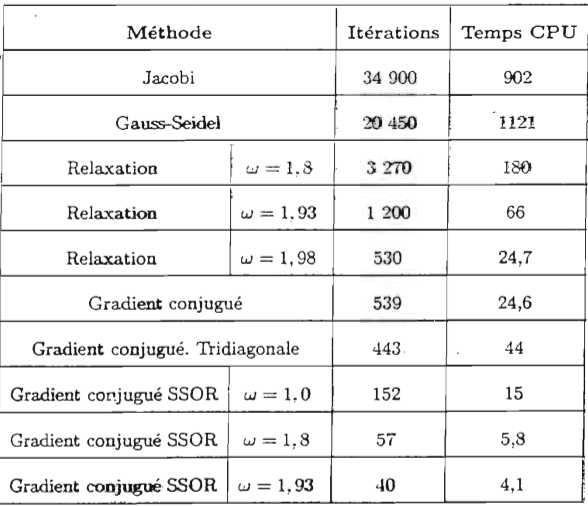
\includegraphics[scale=0.5]{tableau.png}
    \caption{Exemples pratiques}
    \label{fig:tableau}
\end{figure}

